\documentclass{article}

\usepackage{amsmath}
\usepackage{hyperref} 
\usepackage{listings}
\usepackage{graphicx}
\usepackage[margin=1in]{geometry}

\hypersetup{
    colorlinks=true,      
    urlcolor=magenta
}

\usepackage{xcolor}
\lstset {
    backgroundcolor=\color{black!5},
    belowcaptionskip=1\baselineskip,
    breaklines=true,
    frame=L,
    xleftmargin=\parindent,
    language=C++,
    showstringspaces=false,
    basicstyle={\footnotesize}\ttfamily,
    keywordstyle=\bfseries\color{green!40!black},
    commentstyle=\itshape\color{purple!40!black},
    identifierstyle=\color{blue},
    stringstyle=\color{orange}
}

\title{Implementation of nCr for big values of n}
\author{Samyak Ahuja}

\begin{document}

\maketitle

\section{Introduction}
$nCr$ is the coefficient of the $x^r$ term in the polynomial
expansion of $(1+x)^n$ and is given by the formula
\[
    \binom{n}{r} = \frac{n!}{r!(n-r)!}
\]
To calculate $nCr$ one can find the prime factors of $n!$, $r!$, 
and $(n-r)!$ and then cancel out the terms. So in essence all we
have to do is find the powers of the prime factors of the above 
mentioned factorials and then subtract the powers of prime factors 
of $r!$ and $(n-r)!$ from that of $n!$

\vspace{0.2in}

As an example
\begin{align*}
\binom{5}{3} &= \frac{5!}{3!2!} \\\\
&= \frac{5.4.3.2.1}{3.2.1 * 2.1}\\\\
&= \frac{2^3.3^1.5^1}{2^2.3^1}\\\\
&= 2^1.5^1
\end{align*}

One can verify last equation at
\href{https://www.hackmath.net/en/calculator/n-choose-k}{hackmath}

\section{Proof of Correctness}

How do we know that the answer obtained is correct? One can always
calculate it but it isn't practical. On the other hand giving a
rigorous proof requires knowledge of Number Theory. 

Perhaps the best way of going about this is by proving that
the algorithm results in an integer, that is no power of any 
prime factor is negative.

In $nCr$ we have

\[
    \binom{n}{r} = \frac{n!}{r!(n-r)!}
\]

Now a key observation here is that the sum of the numbers that we are
taking the factorial of in the denominator is exactly equal to the 
number in the numberator of which we are taking the factorial. Meaning
$n = r + (n - r)$. So we can if prove generally that

\begin{align*}
     \frac{(n_1 + ... + n_k)!}{n_1!...n_k!}
\end{align*}
is an integer(which can be proved by Lagrange's theorem)
then we can conclude the nCr proof. 

\section{Code}

\lstinputlisting[language=c++]{ncr.cpp}

\vspace{2em}

\section{Output}
\vspace{2em}
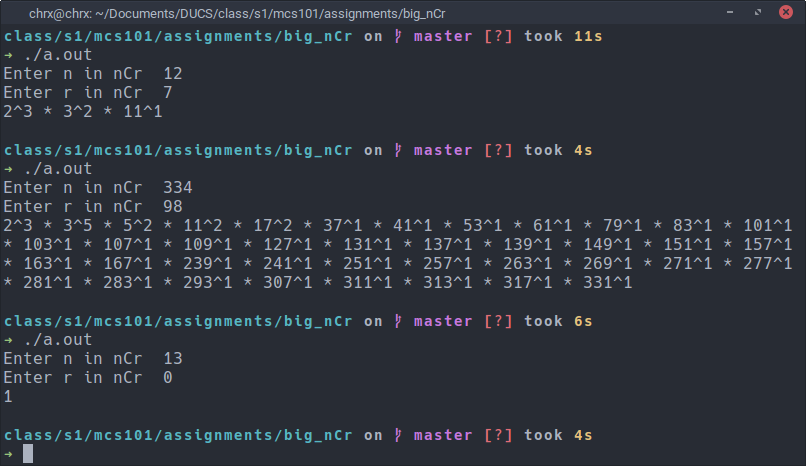
\includegraphics[width = \textwidth]{sc1.png} \\\\ \\\\

\includegraphics[width = \textwidth]{sc2.png}


\section{Runtime}

RunTime of the algorithm in the worst cast is $O(n\sqrt{n})$ where
n is the $n$ in $nCr$ or $\binom{n}{r}$. The run time can be validated
by observing that for a number $n$ we find all the prime numbers upto
$n$ which takes $n.O(\sqrt{n}) = O(n\sqrt{n})$ time. Now for numbers : 
$n$, $r$, and $n-r$ we calculate the powers of prime factors that
constitute towards $n!$, $r!$, and $(n-r)!$ respectively. This is
done in the function \emph{fact} of the code and takes $O(logn)$ in
the worst case. At last subtracting the powers of the prime factors
take $\theta(n)$ time. Hence the entire algorithm runs in 
$O(n\sqrt{n})$ time.

\end{document}